\documentclass[tikz,border=6pt]{standalone}
\usetikzlibrary{arrows.meta,positioning,calc,fit}
\makeatletter
\AtBeginDocument{\global\let\pgf@selectfontorig\relax}
\makeatother

\tikzset{
  state/.style={
    draw=black,
    rounded corners=4pt,
    very thick,
    fill=white,
    minimum width=8.5mm,
    minimum height=7mm,
    align=center,
    inner sep=1.6pt,
    font=\scriptsize
  },
  initial/.style={-Latex, very thick},
  edge/.style={-Latex, thick, shorten >=2pt, shorten <=2pt},
  labelbox/.style={inner sep=3pt, font=\tiny, scale=0.62, transform shape, align=center},
  panel/.style={draw=gray!70, rounded corners=6pt, very thick}
}

\newcommand{\initarrow}[2]{\draw[initial] #1 to (#2);}
\newcommand{\panel}{\draw[panel] (-1.65,-2.65) rectangle (5.85,2.25);}

\begin{document}
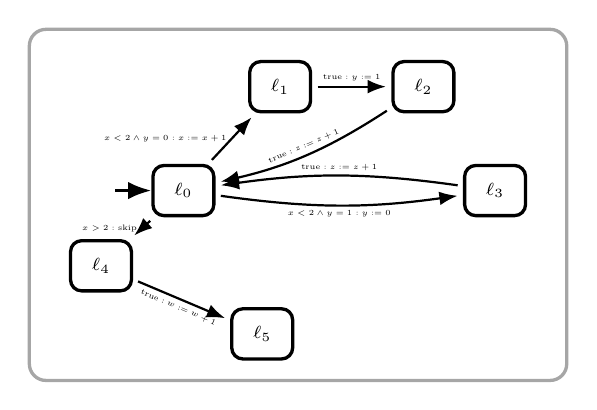
\begin{tikzpicture}[scale=0.91, transform shape]
  \begin{scope}[shift={(.5,0)}]
    \node[state] (p40) at (0,0) {$\ell_0$};
    \node[state] (p41) at (1.35,1.45) {$\ell_1$};
    \node[state] (p42) at (3.35,1.45) {$\ell_2$};
    \node[state] (p43) at (4.35,0) {$\ell_3$};
    \node[state] (p44) at (-1.15,-1.05) {$\ell_4$};
    \node[state] (p45) at (1.1,-2.0) {$\ell_5$};
    \initarrow{(-0.95,0)}{p40.west}
    \draw[edge]                (p40) to node[labelbox, left] {$x<2\land y=0:x:=x+1$} (p41);
    \draw[edge]                (p41) to node[labelbox, above] {$\mathrm{true}:y:=1$} (p42);
    \draw[edge, bend left=10]  (p42) to node[labelbox, above, sloped] {$\mathrm{true}:z:=z+1$} (p40);
    \draw[edge, bend right=8]  (p40) to node[labelbox, below] {$x<2\land y=1:y:=0$} (p43);
    \draw[edge, bend right=8]  (p43) to node[labelbox, above] {$\mathrm{true}:z:=z+1$} (p40);
    \draw[edge]                (p40) to node[labelbox, left] {$x>2:\mathrm{skip}$} (p44);
    \draw[edge]                (p44) to node[labelbox, below, sloped] {$\mathrm{true}:w:=w+1$} (p45);
  \end{scope}
  \panel
\end{tikzpicture}
\end{document}
